% =====================================================================
% Semana 1 · S1.1 — Ley de Ohm mediante barridos
% Fundamentos de Sistemas Electrónicos Analógicos (Ingeniería Aeroespacial)
% Compilar: pdflatex semana_1_s11_ley_ohm.tex  (2 pasadas)
% =====================================================================
\documentclass[aspectratio=169]{beamer}

\usepackage[utf8]{inputenc}
\usepackage[T1]{fontenc}
\usepackage{lmodern}
\usepackage[spanish,es-tabla]{babel}
\usepackage{amsmath,amssymb}
\usepackage{siunitx}
\usepackage{booktabs}
\usepackage{microtype}
\usepackage{circuitikz}

\definecolor{navy}{RGB}{23,54,93}
\definecolor{navysoft}{RGB}{72,101,140}
\definecolor{gold}{RGB}{179,142,62}
\definecolor{ink}{RGB}{44,51,58}
\definecolor{soft}{RGB}{244,241,234}

\usetheme{default}
\setbeamertemplate{navigation symbols}{}
\setbeamertemplate{footline}[frame number]
\setbeamercolor{structure}{fg=navy}
\setbeamercolor{frametitle}{fg=white,bg=navy}
\setbeamercolor{title}{fg=navy}
\setbeamercolor{subtitle}{fg=navysoft}
\setbeamercolor{itemize item}{fg=gold}
\setbeamercolor{itemize subitem}{fg=gold}
\setbeamercolor{block title}{fg=white,bg=navy}
\setbeamercolor{block body}{bg=soft}
\setbeamercolor{example text}{fg=navy}
\setbeamertemplate{itemize item}{\scriptsize\raise1.25pt\hbox{\donotcoloroutermaths$\bullet$}}
\setbeamertemplate{itemize subitem}{\scriptsize\raise1.25pt\hbox{\donotcoloroutermaths$\circ$}}
\setbeamerfont{frametitle}{size=\large,series=\bfseries}

\title[S1.1 · Ley de Ohm]{Ley de Ohm mediante barridos}
\subtitle{S1.1 — Simulaciones y laboratorio de la Semana 1}
\institute{Licenciatura en Ingeniería Aeroespacial\\ UNAM · ENES Unidad Juriquilla}
\author{M. en C. José de Jesús Santana Ramírez}
\date{Semestre 2027-1}

\begin{document}

% ---------------------------------------------------------------------
\begin{frame}[plain]
  \titlepage
\end{frame}

% ---------------------------------------------------------------------
\begin{frame}{Objetivos de la sesión}
  \begin{itemize}
    \item Verificar la \textbf{Ley de Ohm} ($V = I\cdot R$) mediante un barrido de tensión.
    \item Graficar $I$ contra $V$ y comprobar que la \textbf{pendiente es la conductancia} $G = 1/R$.
    \item Comparar las pendientes de $1\,\text{k}\Omega$, $2.2\,\text{k}\Omega$ y $4.7\,\text{k}\Omega$.
    \item Mostrar que la \textbf{potencia crece con el cuadrado} de la tensión: $P = V^2/R$.
    \item Conectar este resultado con el balance de potencia de S1.2.
  \end{itemize}
  \pause
  \begin{block}{Pregunta inicial}
    Si la tensión se duplica, ¿qué ocurre con la corriente y con la potencia?
  \end{block}
\end{frame}

% ---------------------------------------------------------------------
\begin{frame}{Teoría 1 · Ley de Ohm y conductancia}
  \begin{center}
    \resizebox{0.5\linewidth}{!}{%
    \begin{circuitikz}[american voltages, scale=0.95]
      \draw (0,3) to[V, l={$V$}, i=$I$] (0,0);
      \draw (0,3) -- (1.4,3) to[R, l={$R$}] (4.6,3);
      \draw (4.6,3) -- (5.6,3) -- (5.6,0) -- (0,0);
      \node[ground] at (0,0) {};
    \end{circuitikz}}
  \end{center}
  \[
    V = I\cdot R
    \qquad\Longleftrightarrow\qquad
    I = \frac{1}{R}\,V = G\,V
  \]
  \pause
  \begin{itemize}
    \item La corriente es \textbf{lineal} con $V$; la pendiente de $I$ vs $V$ es la
      \textbf{conductancia} $G = 1/R$ (en siemens).
    \item A menor resistencia, mayor pendiente (más corriente) y mayor conductancia.
  \end{itemize}
\end{frame}

% ---------------------------------------------------------------------
\begin{frame}{Profundización · ¿Qué es la conductancia?}
  \begin{block}{Definición}
    La conductancia $G$ es la \textbf{inversa} de la resistencia y mide la
    \emph{facilidad} con que un componente deja pasar la corriente:
    \[
      G = \frac{1}{R}
      \qquad\Longrightarrow\qquad
      I = G\cdot V
    \]
  \end{block}
  \begin{itemize}
    \item \textbf{Unidad:} siemens (S) = amperio por voltio (A/V). Para resistores
      típicos se usa el \emph{millisiemens} (mS).
    \item \textbf{Interpretación física:} $G$ dice cuántos amperios circulan por cada
      voltio aplicado.
      \begin{itemize}
        \item Alta conductancia (baja $R$) $\Rightarrow$ pasa mucha corriente.
        \item Baja conductancia (alta $R$) $\Rightarrow$ pasa poca corriente.
      \end{itemize}
    \item \textbf{En los circuitos:} $G$ es la \textbf{pendiente de la recta} $I$ vs $V$
      (lo que viste en la gráfica de S1.1).
  \end{itemize}
\end{frame}

% ---------------------------------------------------------------------
\begin{frame}{Profundización · Conductancia en paralelo y ejemplo}
  \begin{itemize}
    \item \textbf{En paralelo las conductancias se suman} (conecta con S1.3):
      \[
        G_{total} = G_1 + G_2 + G_3
        \qquad
        R_{eq} = \frac{1}{G_{total}}
        \quad \Rightarrow \quad R_{eq} < R_{mín}
      \]
    \item \textbf{Valores del barrido de S1.1} (pendientes de la gráfica):
      \begin{itemize}
        \item $R = 1\,\text{k}\Omega$ $\Rightarrow$ $G = 1\,\text{mS}$ (la más empinada).
        \item $R = 2.2\,\text{k}\Omega$ $\Rightarrow$ $G = 0.455\,\text{mS}$.
        \item $R = 4.7\,\text{k}\Omega$ $\Rightarrow$ $G = 0.213\,\text{mS}$ (la menos empinada).
      \end{itemize}
    \item Resistencia y conductancia son \textbf{dos vistas del mismo componente}:
      $R$ mide la oposición, $G$ la facilidad; $R = 1/G$.
  \end{itemize}
\end{frame}

% ---------------------------------------------------------------------
\begin{frame}{Teoría 2 · Potencia: parabola, no recta}
  \[
    P = V\cdot I = I^2\,R = \frac{V^2}{R}
  \]
  \pause
  \begin{itemize}
    \item Aunque $I$ es lineal con $V$, la \textbf{potencia crece con $V^2$}.
    \item Duplicar $V$ $\Rightarrow$ el doble de corriente y $\approx 4\times$ la potencia.
    \item Este es el origen del \textbf{límite de derating} (S1.4) y del requisito de
      \textbf{balance de potencia} (S1.2): la potencia no se reparte linealmente.
  \end{itemize}
\end{frame}

% ---------------------------------------------------------------------
\begin{frame}{Ejercicio · Enunciado}
  \begin{block}{Barrido de tensión de la simulación S1.1}
    \centering
    $V_{in}$: de \SI{0}{\volt} a \SI{12}{\volt}; \quad resistores de $1\,\text{k}\Omega$, $2.2\,\text{k}\Omega$ y $4.7\,\text{k}\Omega$.
  \end{block}
  \begin{center}
    \resizebox{0.5\linewidth}{!}{%
    \begin{circuitikz}[american voltages, scale=0.95]
      \draw (0,3) to[V, l={$V_{in}=0\to 12\,\mathrm{V}$}, i=$I$] (0,0);
      \draw (0,3) -- (1.4,3) to[R, l={$R$}] (4.6,3);
      \draw (4.6,3) -- (5.6,3) -- (5.6,0) -- (0,0);
      \node[ground] at (0,0) {};
    \end{circuitikz}}
  \end{center}
  \textbf{Determinar:} la corriente y la potencia para cada resistencia en varios puntos
  del barrido, y explicar por qué la pendiente de $I$ vs $V$ es la conductancia.
\end{frame}

% ---------------------------------------------------------------------
\begin{frame}{Resultado de la simulación}
  \begin{center}
    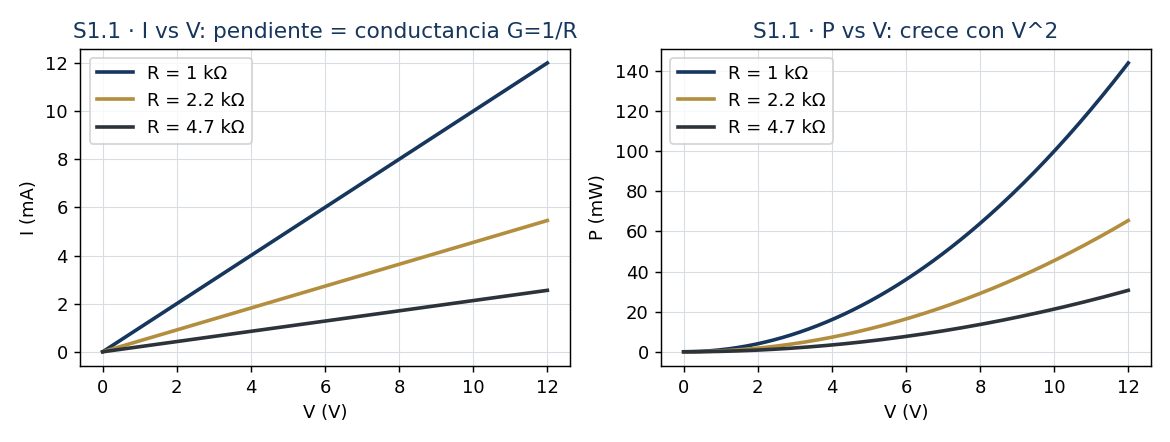
\includegraphics[width=0.86\textwidth]{figs/s11_ohm.png}
  \end{center}
  \begin{itemize}
    \item $I$ vs $V$: rectas cuya pendiente es $G = 1/R$ (la menor resistencia tiene mayor pendiente).
    \item $P$ vs $V$: parábolas: la potencia crece con el cuadrado de la tensión.
  \end{itemize}
\end{frame}

% ---------------------------------------------------------------------
\begin{frame}{Errores comunes}
  \begin{table}
    \small
    \begin{tabular}{p{0.34\textwidth}p{0.30\textwidth}p{0.30\textwidth}}
      \toprule
      Error & Consecuencia & Corrección \\
      \midrule
      Asumir que $P$ crece linealmente con $V$ & Subestimar la disipación & $P = V^2/R$ \\
      Confundir pendiente con resistencia & Curva mal leída & Pendiente de $I$ vs $V$ = conductancia \\
      No anotar unidades & Balance incoherente & Toda magnitud con unidad \\
      Olvidar que $I$ y $P$ cambian con $R$ & Comparar curvas mal & Comparar en el mismo $V$ \\
      \bottomrule
    \end{tabular}
  \end{table}
\end{frame}

% ---------------------------------------------------------------------
\begin{frame}{Preguntas de verificación}
  \begin{enumerate}
    \item Si $V$ se duplica, ¿qué pasa con $I$ y con $P$?
      \uncover<2->{\emph{($I$ se duplica; $P$ se multiplica por 4.)}}
    \item ¿Qué pendiente tiene la curva $I$ vs $V$ de un resistor?
      \uncover<3->{\emph{(La conductancia $G=1/R$.)}}
    \item ¿Cuál conduce más corriente a 5 V: $1\,\text{k}\Omega$ o $4.7\,\text{k}\Omega$?
      \uncover<4->{\emph{($1\,\text{k}\Omega$: menos resistencia, más corriente.)}}
    \item ¿Por qué la potencia crece con $V^2$ y no con $V$?
    \item ¿Cómo se relaciona esta curva con el límite de derating de S1.4?
  \end{enumerate}
\end{frame}

\end{document}
